\documentclass{article}
\usepackage{graphicx} % Required for inserting images
\usepackage{xcolor}
\usepackage{listings}
\usepackage{geometry}
\definecolor{mGreen}{rgb}{0,0.6,0}
\definecolor{mGray}{rgb}{0.5,0.5,0.5}
\definecolor{mPurple}{rgb}{0.58,0,0.82}
\definecolor{backgroundColour}{rgb}{0.95,0.95,0.92}
\usepackage{tikz}
\usepackage{pgfplots}
\usepackage{booktabs}
%https://tex.stackexchange.com/questions/348651/c-code-to-add-in-the-document
\lstdefinelanguage{CMPI}{%
  language     = C,
  morekeywords = {MPI_Reduce},
}
\lstdefinestyle{CStyle}{
    backgroundcolor=\color{backgroundColour},   
    commentstyle=\color{mGreen},
    keywordstyle=\color{magenta},
    numberstyle=\tiny\color{mGray},
    stringstyle=\color{mPurple},
    basicstyle=\footnotesize,
    breakatwhitespace=false,         
    breaklines=true,                 
    captionpos=b,                    
    keepspaces=true,                                  
    showspaces=false,                
    showstringspaces=false,
    showtabs=false,                  
    tabsize=2,
    language=CMPI
}
\pgfplotsset{compat=1.18} 

\usepackage{xcolor}
\title{Gaussian Elimination Determinants}
\author{Albert Luckas}
\date{May 2025}
\begin{document}

\maketitle
\section{Introduction}
The determinant of a matrix is a scalar value associated with the 2-d array, which keeps some of its properties. For example, the product of the determinants of two Matricies is equal to the determinant of their product. Determinants may be used to check if  system of equations has a solution, or if a group of vectors is coplanar. For $2x2$ and $3x3$ Matricies, simple algebraic formulas can be used to compute the determinant by hand, but for larger cases, the naive approach can take up to $O(n!)$ time. The best complexity which has been proven to be possible is $O(n^{2.373})$. For our purposeless, the much simpler Gaussian Elimination algorithm, in $O(n^3)$, will suffice, as it is still quite fast for Matricies up to the desired size, and has large iterations that are ideal for parallelization.
\section{Gaussian Elimination}
Gaussian Elimination works by taking advantage of some definitional properties of the determinant: Adding a multiple of one row or column to another does not change the determinant of a matrix, and the determinant of a diagonal matrix is the product of its diagonal entries. By repeatedly using a row to zero out one column in the remaining rows, we convert the matrix into a triangular matrix with the same determinant. We can then simply multiply down the diagonal, as the conversion to a diagonal matrix would only affect the values above it. \\\\
\begin{figure}
$$
\left|\left(\begin{array}{cccc}
2&4&2&8\cr
1&0&5&2\cr
4&4&5&20\cr
0&4&-1&5\cr
\end{array} \right)\right|
=
\left|\left(\begin{array}{cccc}
2&4&2&8\cr
0&-2&4&-2\cr
0&-4&1&4\cr
0&4&-1&5\cr
\end{array} \right)\right|
=
\left|\left(\begin{array}{cccc}
2&4&2&8\cr
0&-2&4&-2\cr
0&0&-7&8\cr
0&0&7&1\cr
\end{array} \right)\right|
$$
$$
=
\left|\left(\begin{array}{cccc}
2&4&2&8\cr
0&-2&4&-2\cr
0&0&-7&8\cr
0&0&0&9\cr
\end{array} \right)\right|
=
2*-2*-7*9
=252
$$
\caption{An example gaussian elimination on a $4*4$ Matrix}
\end{figure}
In figure 1, we perform an example gaussian elimination on a $4x4$ integer matrix. We first use the top row to set the rest of the first column to zero. We subtract half of it from row 2, double it from row 3, and leave row 4, as it already has the desired $0$. In the second step, we subtract twice row 2 from row 3, and add double row 2 to row 4. Finally, we add row 3 to row 4, giving us an upper diagonal matrix with the same determinant as the original. While wo could continue to get a diagonal matrix, it would not change the result, so we simply multiply down the diagonal and get the result of 252. Of course, the matrices worked on by the computer will not be quite so small, and will consist of floating point numbers instead of integers.
\section{Implementation}
We first make a serial algorithm to compute the gaussian determinant. This works in much the same way as the hand calculation version. The most notable difference is that it keeps a running product of the determinant, instead of waiting for the end. It also keeps track of the log of the determinant, as it may be to large to fit in a floating point number. The middle loop iterates over all the following rows, eliminating their leading element. the innermost loop iterates over their columns to complete the row operation.
\begin{lstlisting}[style=CStyle]
for (int pivot = 0; pivot < size; pivot++)
    {
        logd+=log10(fabs(m[pivot][pivot]));
        d*=m[pivot][pivot];
        for (int r = pivot+1; r < size; r++)
        {
            double mult=m[r][pivot]/m[pivot][pivot];
            for(int c=pivot;c<size;c++){
                m[r][c]-=m[pivot][c]*mult;
            }
        }
        
    }
\end{lstlisting}
Before we parallelize the algorithm, we extract the innermost loop to its own function. The "apply" function uses the pivot row to zero out the "pivot"th element of the target row. The repeated application of this function will can be used to zero out all elements below the diagonal of the matrix.
\begin{lstlisting}[style=CStyle]
void apply(int pivot, int target){
    double mult=m[target][pivot]/m[pivot][pivot];
            for(int c=pivot;c<size;c++){
                m[target][c]-=m[pivot][c]*mult;
            }
}
\end{lstlisting}
I elected to use Pthreads for the parallelization, because it allows the number of threads to be set at runtime, meaning I can pass it as a command line argument to automate testing. It was also extremely important to have shared memory between threads, as otherwise the message passing could easily take the majority of the time.
For the parallel algorithm, we move the loop over the targets above the loop over the pivots. While this is certainly intuitive, it is equivalent, and allows for better parallelism.
\begin{lstlisting}[style=CStyle]
for (int target = rank; target < size; target+=threads)
    {
        for (int pivot = 0; pivot < target; pivot++)
        {
            //printf("waiting for finish of row %i in thread %i\n",pivot,rank);
            pthread_mutex_lock(&done[pivot]);
            pthread_mutex_unlock(&done[pivot]);
            apply(pivot,target);
            //printf("in thread %i, row %i to row %i\n", *rank,pivot,target);
        }
        pthread_mutex_unlock(&done[target]);
        //printf("done doing %i in thread %i\n",target,rank);
         logd+=log10(fabs(m[target][target]));
        d*=m[target][target];
        
    }
\end{lstlisting}
This algorithm computes the expected values for the determinant and log of the determinant for all the input files. Full output data is attached.

\section{Performance}
\subsection{Timing}
We again use timer.h to find the wall time taken in the main process. Unlike MPI, there are not quite as many choices to make- we cannot reasonably create the threads and then start the timer. I ran each test 3 times and took the median time to minimize disruption by other tasks.
\begin{lstlisting}[style=CStyle]
#include "timer.h"
...
    double start, finish;
    GET_TIME(start);
    ...  //timed work
    GET_TIME(finish);    
    printf("%f\n",finish-start);
    \end{lstlisting}
\subsection{Performance with One thread}
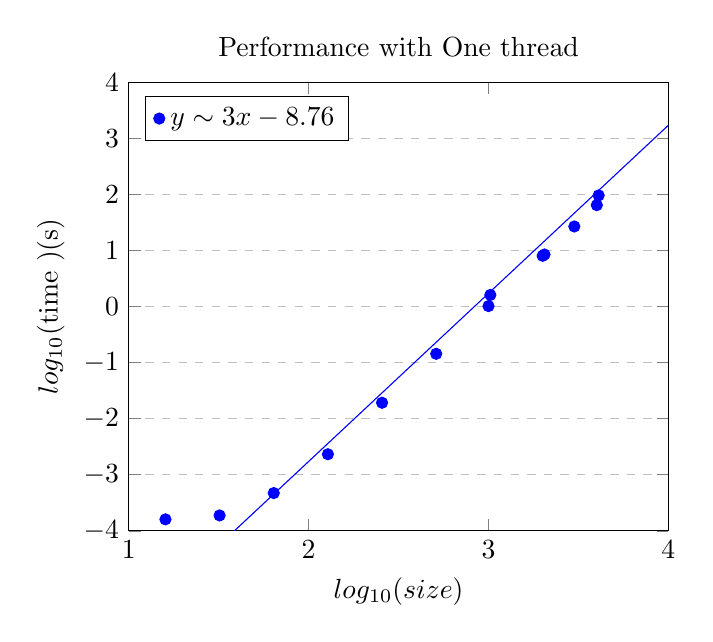
\begin{tikzpicture}
\begin{axis}[
    title={Performance with One thread},
    xlabel={$log_{10}(size)$},
    ylabel={$log_{10}($time $)$(s)},
    xmin=1, xmax=4,
    ymin=-4, ymax=4,
    xtick={0,1,2,3,4,5,6,7,8,9,10},
    ytick={-4,-3,-2,-1,0,1,2,3,4},
    legend pos=north west,
    ymajorgrids=true,
    grid style=dashed,
]

    \addplot[
    color=blue,
    only marks,
    ]
    coordinates {(1.204119983,-3.795880017)(1.505149978,-3.725842151)(1.806179974,-3.326979093)(2.10720997,-2.634137785)(2.408239965,-1.715230987)(2.709269961,-0.8417551453)(3,0.00977373449)(3.010299957,0.2083878726)(3.301029996,0.9067807462)(3.311329952,0.9300963563)(3.477121255,1.430154341)(3.602059991,1.811150826)(3.612359948,1.98445941)
    };
    \addplot[
    color=blue,
    domain=-10:10, 
    ]
    {3*x-8.76324};
    \addlegendentry{\(y\sim 3x-8.76\)}
\end{axis}
\end{tikzpicture} %double-log accuracy : n

For the serial implementation, we get a double-log best fit line with slope 3, consistent with the theoretical complexity of $O(n^3)$. The actual runtime is rather small, with the largest matrix only taking a minute and a half- faster than expected.
\subsection{Performance for constant size matrix}

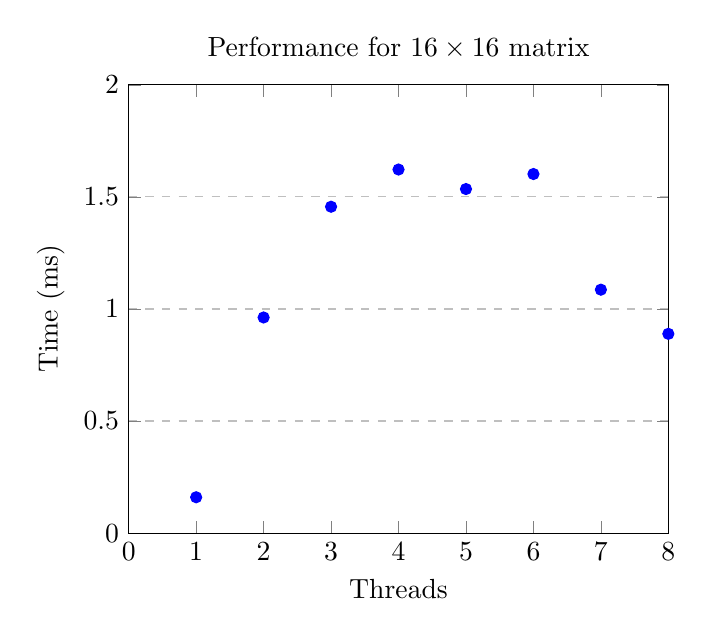
\begin{tikzpicture}
\begin{axis}[
    title={Performance for $16\times16$ matrix},
    xlabel={Threads},
    ylabel={Time (ms)},
    xmin=0, xmax=8,
    ymin=0, ymax=2,
    xtick={0,1,2,3,4,5,6,7,8},
    ytick={0,0.5,1,1.5,2},
    legend pos=north west,
    ymajorgrids=true,
    grid style=dashed,
]

    \addplot[
    color=blue,
    only marks,
    ]
    coordinates {(1,0.16)(2,0.962)(3,1.456)(4,1.622)(5,1.535)(6,1.602)(7,1.086)(8,	0.889)
    };
   
\end{axis}
\end{tikzpicture} %16
\\
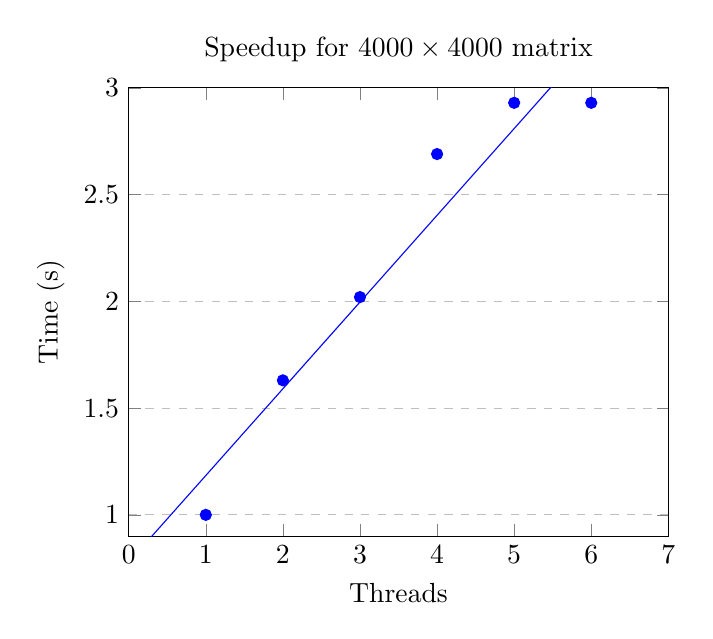
\begin{tikzpicture}
\begin{axis}[
    title={Speedup for $4000\times4000$ matrix},
    xlabel={Threads},
    ylabel={Time (s)},
    xmin=0, xmax=7,
    ymin=0.9, ymax=3,
    xtick={0,1,2,3,4,5,6,7,8},
    ytick={1,1.5,2,2.5,3},
    legend pos=north west,
    ymajorgrids=true,
    grid style=dashed,
]

    \addplot[
    color=blue,
    only marks,
    ]
    coordinates {(1,1.00)
(2,1.63)
(3,2.02)
(4,2.69)
(5,2.93)
(6,2.93)
    };
    
     \addplot[
    color=blue,
    domain=0:8, 
    ]
    {0.406286*x+0.778};
   
\end{axis}
\end{tikzpicture} %speedup
\\
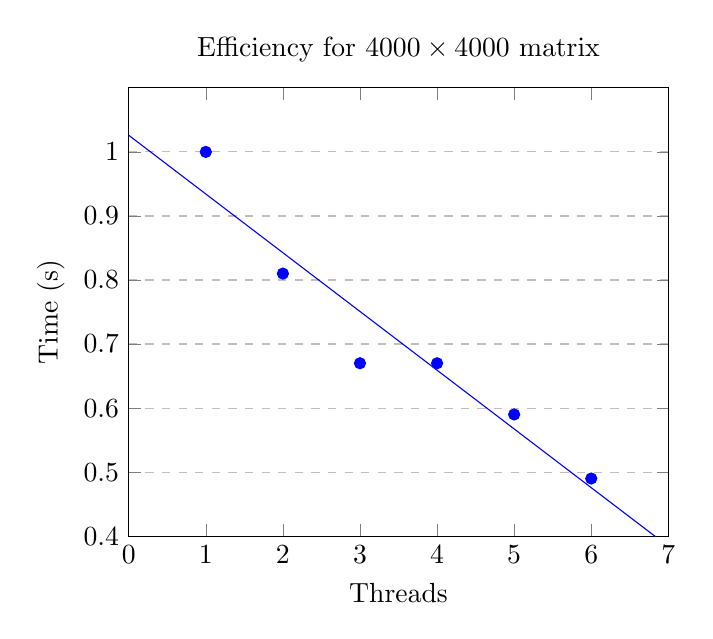
\begin{tikzpicture}
\begin{axis}[
    title={Efficiency for $4000\times4000$ matrix},
    xlabel={Threads},
    ylabel={Time (s)},
    xmin=0, xmax=7,
    ymin=0.4, ymax=1.1,
    xtick={0,1,2,3,4,5,6,7,8},
    ytick={0,0.1,0.2,0.3,0.4,0.5,0.6,0.7,0.8,0.9,1},
    legend pos=north west,
    ymajorgrids=true,
    grid style=dashed,
]

    \addplot[
    color=blue,
    only marks,
    ]
    coordinates {(1,1.00)
(2,0.81)
(3,0.67)
(4,0.67)
(5,0.59)
(6,0.49)
    };
    
     \addplot[
    color=blue,
    domain=0:8, 
    ]
    {-0.0917143*x+1.026};
   
\end{axis}
\end{tikzpicture} %efficiency
\\
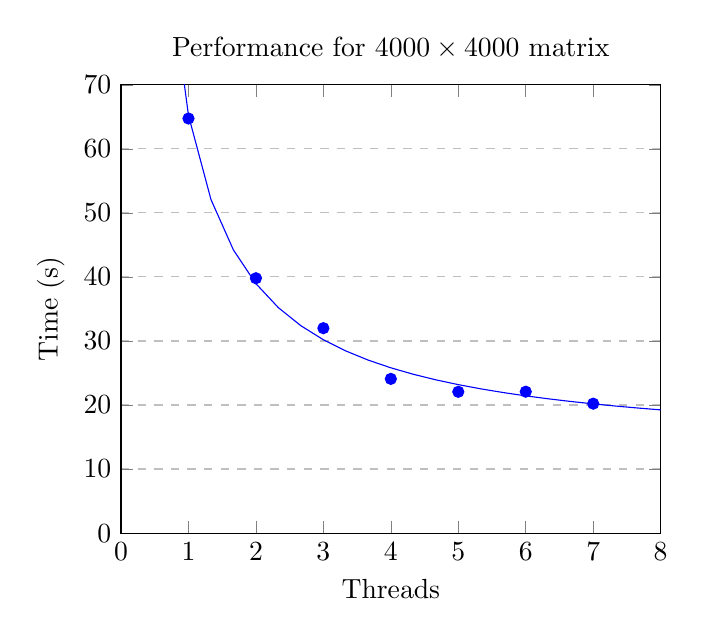
\begin{tikzpicture}
\begin{axis}[
    title={Performance for $4000\times4000$ matrix},
    xlabel={Threads},
    ylabel={Time (s)},
    xmin=0, xmax=8,
    ymin=0, ymax=70,
    xtick={0,1,2,3,4,5,6,7,8},
    ytick={0,10,20,30,40,50,60,70},
    legend pos=north west,
    ymajorgrids=true,
    grid style=dashed,
]

    \addplot[
    color=blue,
    only marks,
    ]
    coordinates {(1,64.73674)(2,39.796963)(3,31.996446)(4,24.07957)(5,22.061285)(6,22.078518)(7,20.209654)
    };
     \addplot[
    color=blue,
    domain=0:8, 
    ]
    {52.55593/x+12.66966};
   
\end{axis}
\end{tikzpicture} %4000
\\
For the small matrix, we see that the program scales very poorly. The overhead from additional threads overwhelms the improvements and makes the parralel version run slower. For a large matrix, however, there is substantial improvement, with efficiency maintained above 50\% up to the number of cores on my machine. The time taken is consistent with an overhead of about 12 seconds, with a $R^2$ value of 0.99 for the line of best fit in form $y=\frac{m}{x}+b$. The speedup is consistently about half the number of cores.
\section{Full Source Code}
All code for the matrix determinant task was written by Albie Luckas
\begin{lstlisting}[style=CStyle]

 #include <stdio.h>
 #include <stdlib.h>
 #include <string.h>
 #include <math.h>
 #include <pthread.h>
 #include "timer.h"
 double d;
 double logd;
 int size;
 double ** m;
 pthread_mutex_t * done;
 void* Thread_work(void* rank);
 void apply(int pivot, int target);
int threads;
 int main(int argc, char const *argv[])
{ 
    
    if(argc!=3){
        printf("usage:%s <size> <threads>\n",argv[0]);
        return 1;
    }
    size=strtol(argv[1],NULL,10);
    threads=strtol(argv[2],NULL,10);
    const char* sizestr=argv[1];
    char fname[21];
    sprintf(fname,"input/m%sx%s.bin",sizestr,sizestr);
    FILE * fp;
    m=malloc(size*sizeof(double*));
    fp = fopen(fname, "r");
    if(NULL==fp){
        printf("error opening file. was size a 4-digit power of 2 or multiple of 1000 between 16 and 5000? ");
        return 2;
    }

    for (int i = 0; i < size; i++)
    {
        m[i]=malloc(size*sizeof(double));
        fread(m[i],sizeof(double),size,fp);
    }
    fclose(fp);
    d=1; 
    logd=0;
    double start, finish;
    GET_TIME(start);

    done=malloc(sizeof(pthread_mutex_t)*size);
    for (int i = 0; i < size; i++)
    {
        pthread_mutex_init(&done[i],NULL);
        pthread_mutex_lock(&done[i]);
    }
    pthread_mutex_unlock(&done[0]);
    
    pthread_t* thread_handles = malloc (threads*sizeof(pthread_t));
     for (int thread = 0; thread < threads; thread++)
       pthread_create(&thread_handles[thread], NULL,
           Thread_work, (void*) thread);
 
    for (int thread = 0; thread < threads; thread++) {
       pthread_join(thread_handles[thread], NULL);
    }
    
    
    
    GET_TIME(finish);




    // free and return
    for (int i = 0; i < size; i++)
    {
        //for (int j = 0; j < size; j++) printf("%lf ",m[i][j]);printf("\n");
        free(m[i]);
    }
    free(m);
    free(done);
    printf("Size:%i\nDetermenant: %lf\nLog(det): %lf\nTime: %f\nThreads:%i \n\n",size, d,logd,finish-start,threads);
    return 0;
}

void* Thread_work(void* in){
    int rank=in;
    //printf("rank:%i\n",*rank);
    for (int target = rank; target < size; target+=threads)
    {
        for (int pivot = 0; pivot < target; pivot++)
        {
            //printf("waiting for finish of row %i in thread %i\n",pivot,rank);
            pthread_mutex_lock(&done[pivot]);
            pthread_mutex_unlock(&done[pivot]);
            apply(pivot,target);
            //printf("in thread %i, row %i to row %i\n", *rank,pivot,target);
        }
        pthread_mutex_unlock(&done[target]);
        //printf("done doing %i in thread %i\n",target,rank);
         logd+=log10(fabs(m[target][target]));
        d*=m[target][target];
        
    }

}

void apply(int pivot, int target){
    double mult=m[target][pivot]/m[pivot][pivot];
            for(int c=pivot;c<size;c++){
                m[target][c]-=m[pivot][c]*mult;
            }
}
\end{lstlisting}

\newgeometry{left=0cm,right=0cm}
\section{Full Data}
\begin{table}[]
    \centering
    \begin{tabular}{|r|r|c||r|r|c||r|r|c|}
    \hline
    threads&size&median time&threads&size&median time&threads&size&median time\\
\hline
1&16&1.60E-04&1&256&1.93E-02&1&1000&1.02E+00\\
2&16&9.62E-04&2&256&1.74E-02&2&1000&8.09E-01\\
3&16&1.46E-03&3&256&1.21E-02&3&1000&4.53E-01\\
4&16&1.62E-03&4&256&1.09E-02&4&1000&3.52E-01\\
5&16&1.54E-03&5&256&1.17E-02&5&1000&3.38E-01\\
6&16&1.60E-03&6&256&1.64E-02&6&1000&4.09E-01\\
7&16&1.09E-03&7&256&2.92E-02&7&1000&3.06E-01\\
8&16&8.89E-04&8&256&2.16E-02&8&1000&3.86E-01\\
10&16&1.19E-03&10&256&2.30E-02&10&1000&2.44E-01\\
16&16&9.50E-04&16&256&4.40E-02&16&1000&2.84E-01\\
32&16&2.36E-03&32&256&6.84E-02&32&1000&4.87E-01\\
64&16&3.50E-03&64&256&1.17E-01&64&1000&1.05E+00\\
\hline
1&32&1.88E-04&1&512&1.44E-01&1&2000&8.07E+00\\
2&32&1.61E-03&2&512&7.51E-02&2&2000&4.85E+00\\
3&32&3.33E-03&3&512&7.95E-02&3&2000&3.71E+00\\
4&32&3.93E-03&4&512&4.76E-02&4&2000&2.83E+00\\
5&32&4.72E-03&5&512&5.28E-02&5&2000&2.82E+00\\
6&32&3.28E-03&6&512&2.81E-02&6&2000&4.16E+00\\
7&32&3.10E-03&7&512&4.45E-02&7&2000&3.63E+00\\
8&32&4.29E-03&8&512&5.62E-02&8&2000&3.62E+00\\
10&32&4.35E-03&10&512&4.71E-02&10&2000&2.25E+00\\
16&32&3.39E-03&16&512&8.48E-02&16&2000&2.11E+00\\
32&32&2.99E-03&32&512&1.46E-01&32&2000&2.24E+00\\
64&32&4.51E-03&64&512&3.28E-01&64&2000&2.82E+00\\
\hline
1&64&4.71E-04&1&1024&1.62E+00&1&3000&2.69E+01\\
2&64&1.25E-03&2&1024&6.40E-01&2&3000&1.61E+01\\
3&64&4.86E-03&3&1024&4.80E-01&3&3000&1.18E+01\\
4&64&5.04E-03&4&1024&7.23E-01&4&3000&9.89E+00\\
5&64&1.05E-02&5&1024&3.40E-01&5&3000&8.73E+00\\
6&64&8.64E-03&6&1024&3.47E-01&6&3000&8.90E+00\\
7&64&6.11E-03&7&1024&3.83E-01&7&3000&8.20E+00\\
8&64&8.27E-03&8&1024&3.10E-01&8&3000&7.92E+00\\
10&64&7.70E-03&10&1024&2.77E-01&10&3000&6.76E+00\\
16&64&7.45E-03&16&1024&3.08E-01&16&3000&7.22E+00\\
32&64&9.66E-03&32&1024&6.37E-01&32&3000&6.98E+00\\
64&64&5.07E-03&64&1024&7.27E-01&64&3000&7.78E+00\\
\hline
1&128&2.32E-03&1&2048&8.51E+00&1&4000&6.47E+01\\
2&128&2.04E-03&2&2048&5.26E+00&2&4000&3.98E+01\\
3&128&4.58E-03&3&2048&3.65E+00&3&4000&3.20E+01\\
4&128&8.41E-03&4&2048&3.18E+00&4&4000&2.41E+01\\
5&128&7.49E-03&5&2048&3.16E+00&5&4000&2.21E+01\\
6&128&1.60E-02&6&2048&2.78E+00&6&4000&2.21E+01\\
7&128&9.18E-03&7&2048&2.68E+00&7&4000&2.02E+01\\
8&128&9.02E-03&8&2048&3.39E+00&8&4000&2.84E+01\\
10&128&1.59E-02&10&2048&2.77E+00&10&4000&1.61E+01\\
16&128&1.67E-02&16&2048&2.11E+00&16&4000&1.58E+01\\
32&128&2.93E-02&32&2048&2.39E+00&32&4000&1.53E+01\\
64&128&2.28E-02&64&2048&5.55E+00&64&4000&1.63E+01\\
\hline
1&4096&9.65E+01&5&4096&2.38E+01&10&4096&1.95E+01\\
2&4096&4.18E+01&6&4096&2.24E+01&16&4096&2.77E+01\\
3&4096&3.33E+01&7&4096&2.25E+01&32&4096&1.80E+01\\
4&4096&2.81E+01&8&4096&3.04E+01&64&4096&2.08E+01\\
\hline
    \end{tabular}
    \caption{Median Runtimes in Seconds}
    \label{tab:my_label}
\end{table}




\end{document}
